\chapter{Intervalos de valores razonables}

En este apartado diferenciaremos los tipos de intervalos de valores nos permiten cuantificar la variabilidad de los resultados y, por tanto, la incertidumbre de la medición realizada. 

\begin{itemize}

    \item El \textbf{intervalo de confianza (IC)} es una herramienta común de la estadística frecuentista, que permite estimar un rango de valores tal que podamos confiar en que contiene al valor verdadero de un parámetro poblacional desconocido $\theta$ (p.ej., la media) \cite{berrendero2025}.

    Los métodos del cálculo del IC dependen de la distribución del estimador (p.ej., la distribución de la
    media muestral) y los parámetros conocidos. 

    Es importante aclarar un malentendido común: un intervalo de confianza con nivel 95\% para un parámetro $\theta$ no significa que exista un 95\% de probabilidad de que $\theta$ esté dentro del intervalo calculado a partir de una muestra específica. En realidad, el 95\% se refiere a la frecuencia con la que, si muestreásemos muchas veces los datos, los intervalos construidos a partir de esas muestras incluirían al valor verdadero de $\theta$ en aproximadamente el 95\% \cite{murphy2022} (véase la Figura \ref{fig:confidence_interval}).

    \begin{figure}[htbp]
        \centering
        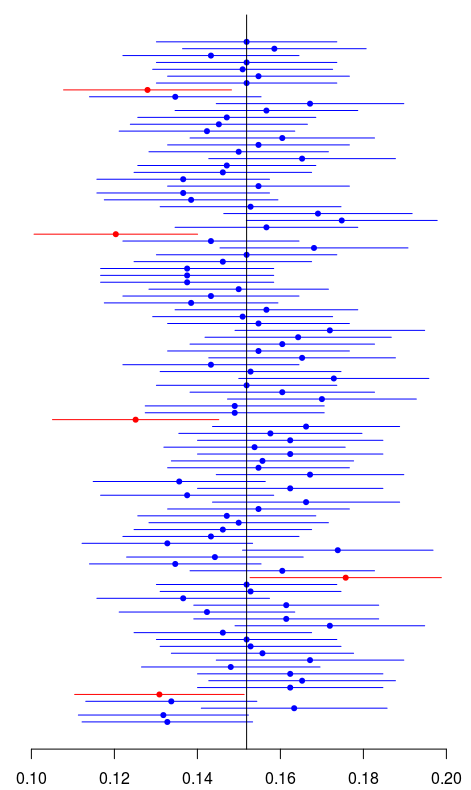
\includegraphics[width=0.55\textwidth]{apendices/imagenes/confidence_interval.png}
        \caption[
            Ejemplo de intervalo de confianza para la media poblacional.
        ]{
            Ejemplo de intervalos de confianza para la media poblacional. La interpretación correcta del nivel de confianza (95\% en este caso) es: \textit{Si repitiéramos el proceso de muestreo y construcción de intervalos muchas veces, aproximadamente el 95\% de ellos contendrían el verdadero valor de la media poblacional}. En esta simulación, la media real conocida es 0.153, y podemos ver que la mayoría de los intervalos la capturan, mientras que unos pocos (generalmente alrededor del 5\%) no lo logran.
            En general, se suele pedir uno solo de estos intervalos, calculado con toda la muestra disponible, aunque la media poblacional podrá estar o no contenida, pero es desconocido. 
        } 
        \label{fig:confidence_interval}
    \end{figure}


    \item El \textbf{intervalo de credibilidad o región creíble (RC)} es, de hecho, la que determina que el parámetro $\theta$ está contenido en el rango de sus valores con una probabilidad determinada por el nivel de credibilidad. Este intervalo es la aproximación bayesiana equivalente al intervalo de confianza, y, como este, requiere conocer la distribución a priori de los datos.

    La diferencia radica en que, a diferencia del intervalo de confianza, que parte de que $\theta$ es un parámetro fijo desconocido y los datos son tratados como aleatorios, el enfoque bayesiano fija los datos(ya que son conocidos) y el parámetro $\theta$ lo trata como aleatorio (ya que es desconocido) \cite{murphy2022}.

    Esta interpretación resulta más intuitiva y directa en comparación con la interpretación frecuentista del intervalo de confianza. En particular, una región creíble del 95\% sí puede interpretarse como que hay un 95\% de probabilidad de que el parámetro $\theta$ se encuentre dentro de ese intervalo, dado el conjunto de datos observado y la distribución a priori asumida.

    \begin{figure}[htbp]
        \centering
        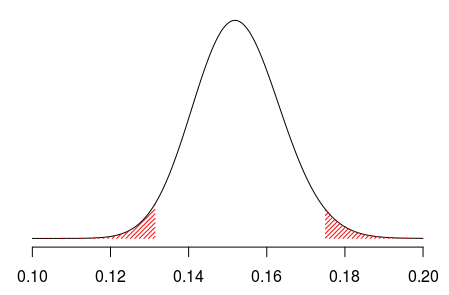
\includegraphics[width=0.75\textwidth]{apendices/imagenes/credibility_interval.png}
        \caption[
            Ejemplo de intervalo de credibilidad para la media poblacional.
        ]{
            Ejemplo de intervalo de credibilidad para la media poblacional. La interpretación correcta es: \textit{Con un 95\% de probabilidad, el valor verdadero está dentro del intervalo}. En esta simulación, la media real conocida es 0.153, y podemos observar que efectivamente este valor está contenido en el intervalo.
        } 
        \label{fig:credibility_interval}
    \end{figure}


    \item El \textbf{intervalo de predicción (\textit{prediction interval})} es radicalmente diferente a los intervalos previos. Trata de predecir un valor futuro de una observación, no determinar un parámetro poblacional. Existen numerosos métodos, con y sin necesidad de conocer la distribución de los datos. 
    
    El enfoque explorado en este trabajo es la predicción conformal, que ha demostrado ser eficaz en contextos donde los supuestos clásicos (normalidad, homocedasticidad) no se cumplen \cite{romano2019}, y es actualmente el enfoque más robusto para la construcción de intervalos de predicción en aplicaciones modernas de ML \cite{romano2019, luo2025, sadinle2019, romano2020, angelopoulos2020}. La predicción conformal tiene una interpretación frecuentista: $1-\alpha$ intervalos producidos cubren el verdadero valor (véase la Figura \ref{fig:prediction_intervals}).

    \begin{figure}[htbp]
        \centering
        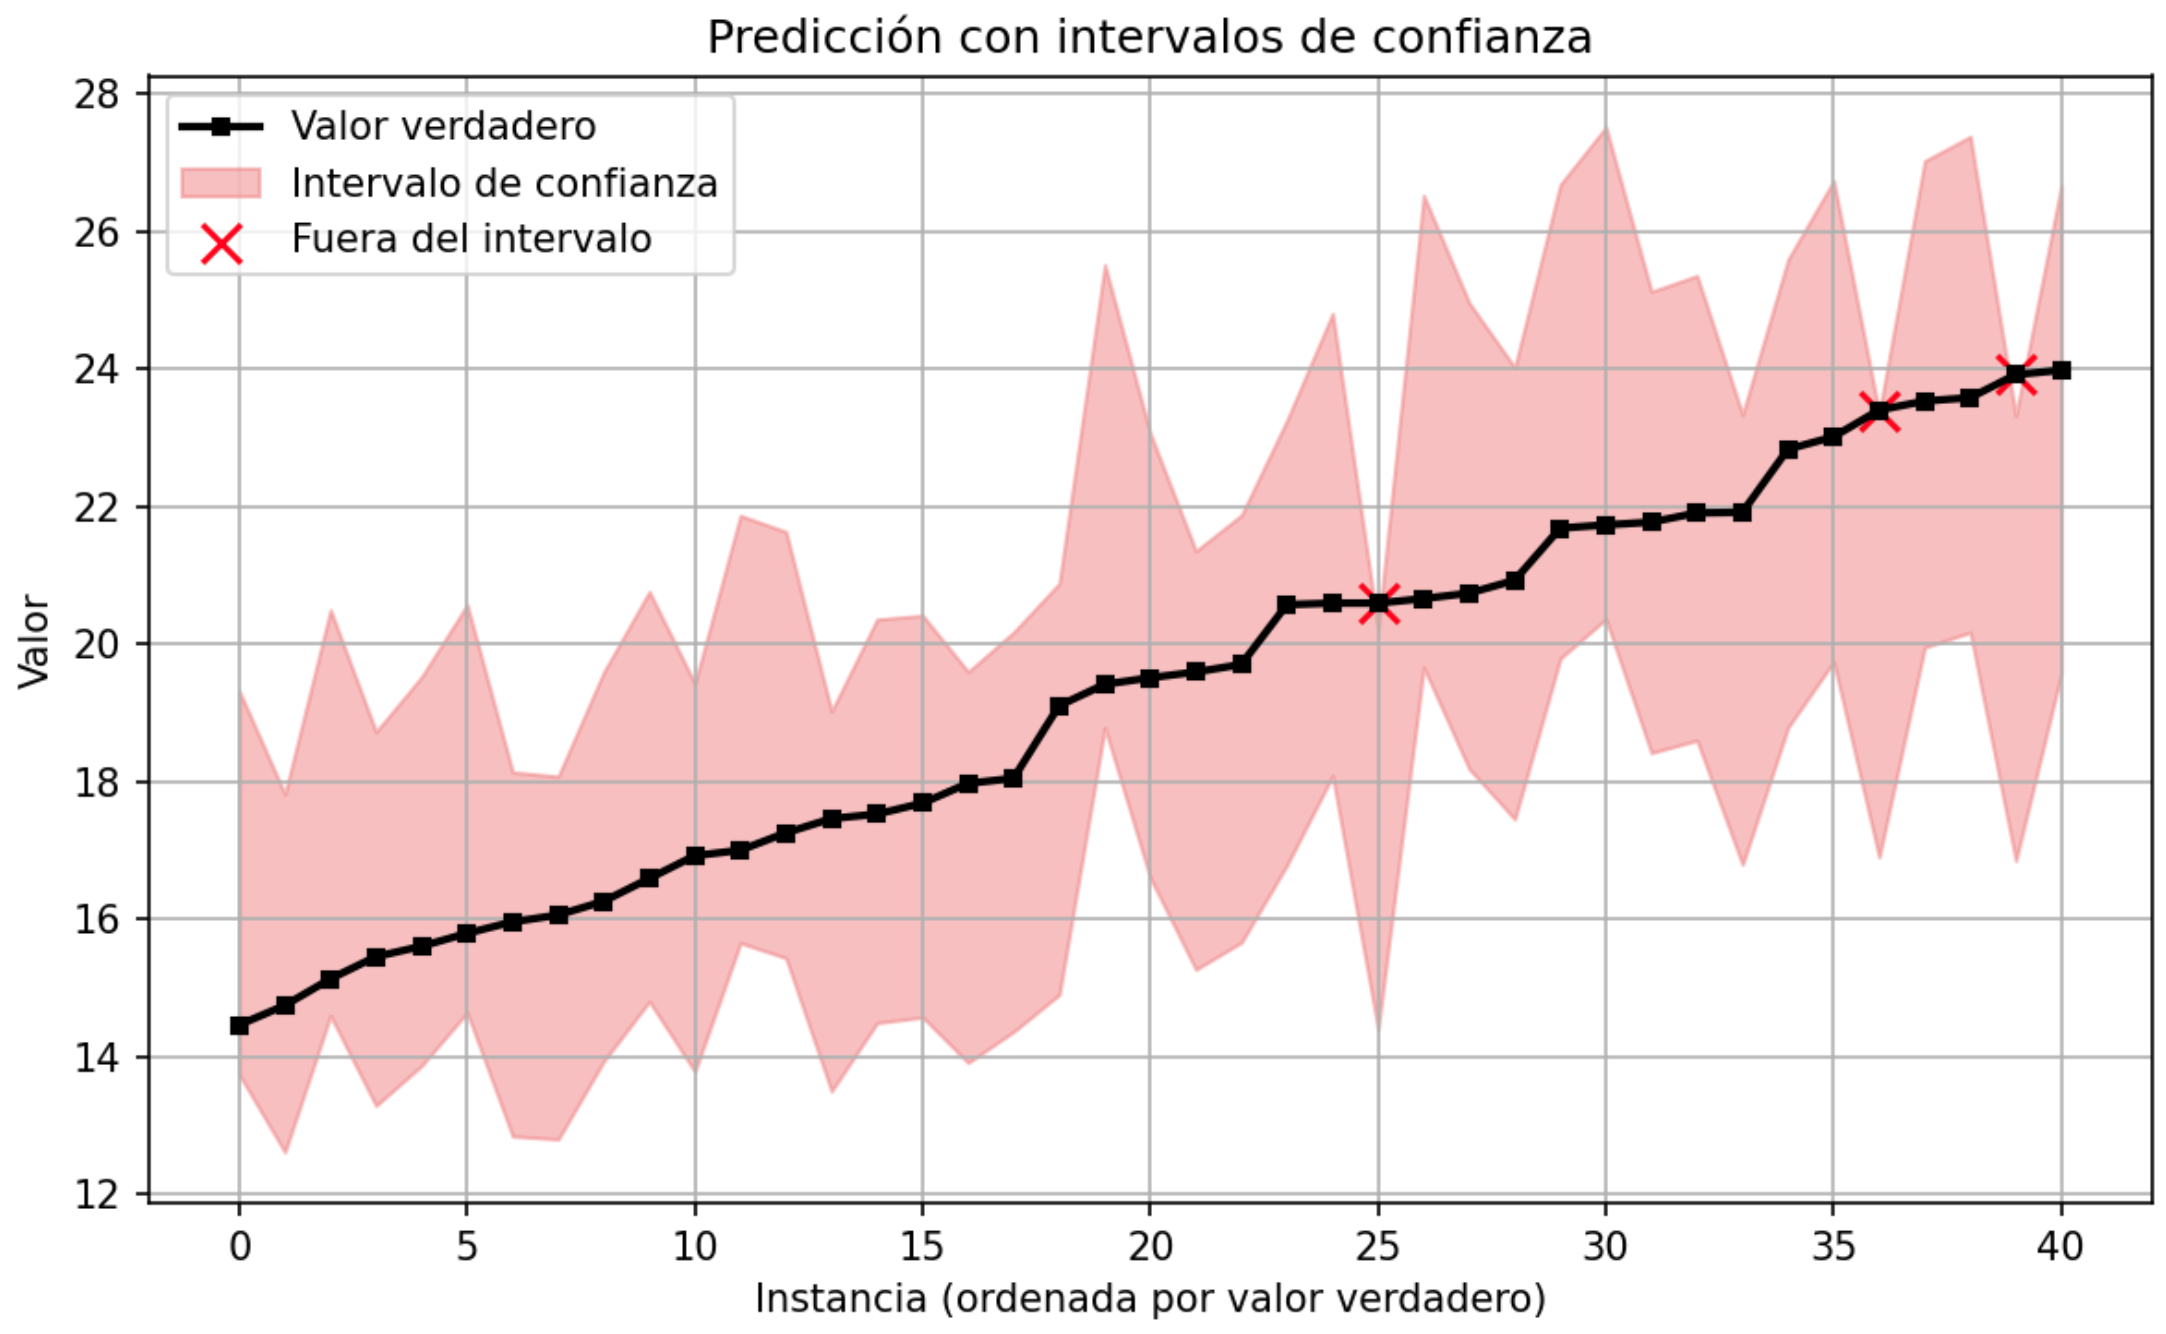
\includegraphics[width=0.75\textwidth]{apendices/imagenes/prediction_intervals.png}
        \caption[
            Intervalos de predicción (95\% de confianza) construidos con CQR para estimación de edad.
        ]{
            Intervalos de predicción (95\% de confianza) construidos con CQR para estimación de edad.
        } 
        \label{fig:prediction_intervals}
    \end{figure}

\end{itemize}

% Relacionándolo con el apartado anterior, los intervalos de confianza solo informan de la incertidumbre 
% aleatoria, puesto que asumen que el modelo está bien especificado y que el error residual es la única fuente 
% de variabilidad. 

% Los intervalos de credibilidad sí integran la incertidumbre en los parámetros del modelo y en la estructura 
% del modelo mismo, capturando así tanto la incertidumbre aleatoria como la incertidumbre epistémica.

% Frente a estos, los intervalos de predicción obtenidos mediante predicción conformal sí presentan información
% de los tres componentes de incertidumbre. 

Como podemos esperar, a más estrecho sea el intervalo que manejemos, más se puede confiar en las predicciones pero no todos los tipos de intervalos revelan la misma información sobre incertidumbre. 